\documentclass{article}
\usepackage{tikz}
\usepackage{pgfplots}
\usepackage{amsmath}
\usepackage[margin=1cm]{geometry}
\usetikzlibrary{shapes,arrows,positioning,calc,decorations.pathreplacing}

\title{Optimal Babbage Analytical Engine Visualizations}
\author{Mechanical Computing Architecture}
\date{1910 Specification Era}

\begin{document}

\maketitle

\section{System Architecture Overview}

\begin{center}
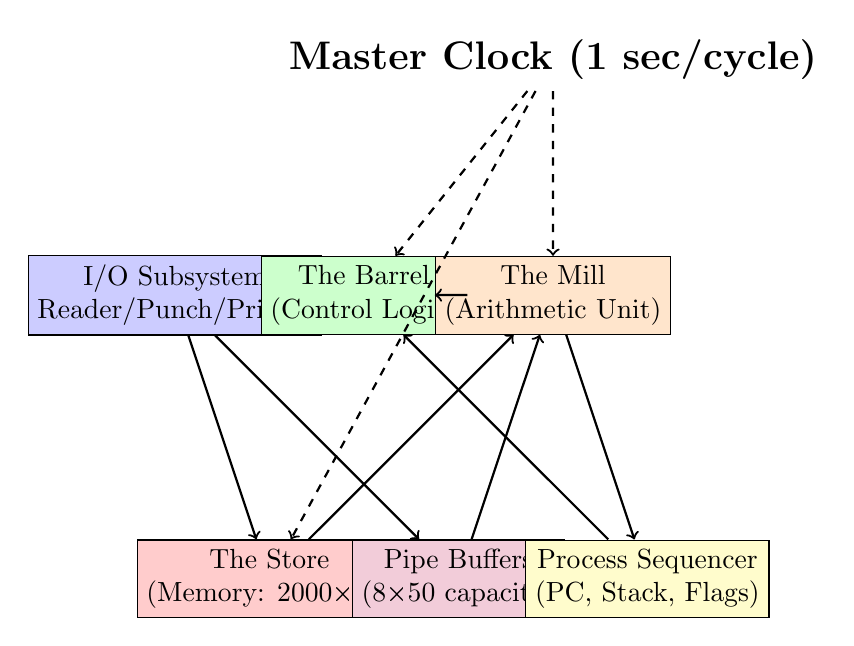
\begin{tikzpicture}[scale=1.2, every node/.style={draw, rectangle, minimum width=2cm, minimum height=0.8cm, align=center}]

% Main components
\node[fill=blue!20] (io) at (0, 8) {I/O Subsystem\\Reader/Punch/Printer};
\node[fill=green!20] (barrel) at (2, 8) {The Barrel\\(Control Logic)};
\node[fill=orange!20] (mill) at (4, 8) {The Mill\\(Arithmetic Unit)};

% Store and pipes
\node[fill=red!20] (store) at (1, 5) {The Store\\(Memory: 2000×50)};
\node[fill=purple!20] (pipes) at (3, 5) {Pipe Buffers\\(8×50 capacity)};
\node[fill=yellow!20] (seq) at (5, 5) {Process Sequencer\\(PC, Stack, Flags)};

% Master clock
\node[draw=none] (clock) at (4, 10.5) {\Large \textbf{Master Clock (1 sec/cycle)}};

% Connections
\draw[->,thick] (io) -- (store);
\draw[->,thick] (barrel) -- (mill);
\draw[->,thick] (mill) -- (seq);
\draw[->,thick] (store) -- (mill);
\draw[->,thick] (seq) -- (barrel);
\draw[->,thick] (pipes) -- (mill);
\draw[->,thick] (io) -- (pipes);

% Clock signal
\draw[->,dashed,thick] (clock) -- (barrel);
\draw[->,dashed,thick] (clock) -- (mill);
\draw[->,dashed,thick] (clock) -- (store);

\end{tikzpicture}
\end{center}

\newpage

\section{The Mill: Arithmetic Unit Architecture}

\begin{center}
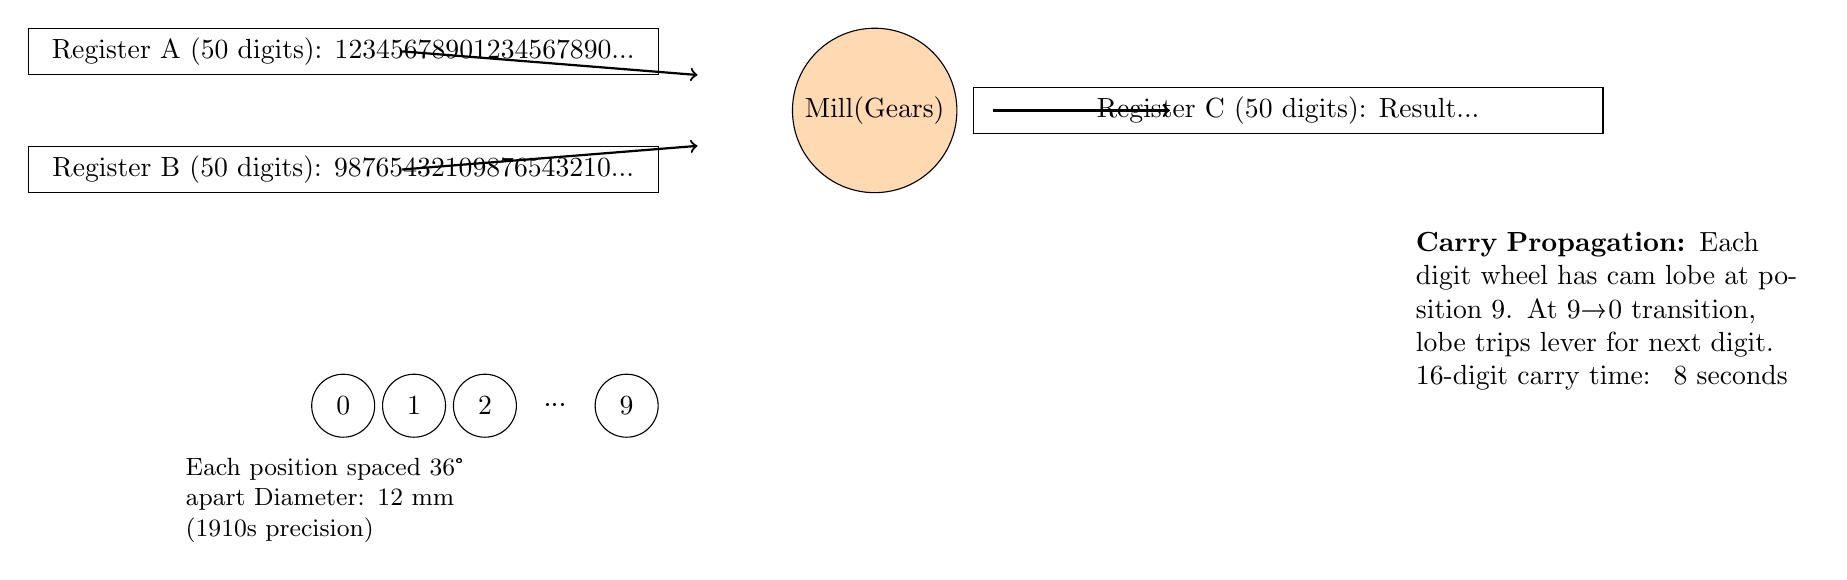
\begin{tikzpicture}[scale=1.5]

% Register A
\node[draw, rectangle, minimum width=8cm, minimum height=0.5cm] (rega) at (0, 3) {Register A (50 digits): 12345678901234567890...};

% Register B
\node[draw, rectangle, minimum width=8cm, minimum height=0.5cm] (regb) at (0, 2) {Register B (50 digits): 98765432109876543210...};

% Central Mill Unit
\node[draw, circle, minimum size=2cm, fill=orange!30] (mill) at (4.5, 2.5) {Mill\\(Gears)};

% Output
\node[draw, rectangle, minimum width=8cm, minimum height=0.5cm] (regc) at (8, 2.5) {Register C (50 digits): Result...};

% Carry mechanism
\draw[->,thick] (0.5, 3) -- (3, 2.8);
\draw[->,thick] (0.5, 2) -- (3, 2.2);
\draw[->,thick] (5.5, 2.5) -- (7, 2.5);

% Carry chain detail
\node at (9, 0.8) [anchor=west, draw=none, text width=5cm] {
\textbf{Carry Propagation:}
Each digit wheel has cam lobe at position 9.
At 9→0 transition, lobe trips lever for next digit.
16-digit carry time: ~8 seconds
};

% Digit wheel detail
\node at (0, 0) [circle, draw, minimum size=0.8cm] {0};
\node at (0.6, 0) [circle, draw, minimum size=0.8cm] {1};
\node at (1.2, 0) [circle, draw, minimum size=0.8cm] {2};
\node[draw=none] at (1.8, 0) {···};
\node at (2.4, 0) [circle, draw, minimum size=0.8cm] {9};

\node at (0, -0.8) [draw=none, text width=4cm, font=\small] {
Each position spaced 36° apart
Diameter: 12 mm (1910s precision)
};

\end{tikzpicture}
\end{center}

\newpage

\section{Digit Wheel Mechanism (Cross-Section)}

\begin{center}
\begin{tikzpicture}[scale=2]

% Wheel cross-section
\draw[fill=gray!20] (0, 0) circle (1cm);
\draw[thick] (0, 0) circle (1cm);

% Tooth positions for digits 0-9
\foreach \i in {0,1,2,3,4,5,6,7,8,9} {
  \pgfmathsetmacro{\angle}{\i * 36}
  \draw[thick] ({\cos(\angle) * 0.9}, {\sin(\angle) * 0.9}) -- ({\cos(\angle) * 1.1}, {\sin(\angle) * 1.1});
  \node at ({\cos(\angle) * 1.3}, {\sin(\angle) * 1.3}) {\i};
}

% Cam lobe at position 9
\draw[fill=red, thick] (1.05, 0.2) -- (1.15, 0.1) -- (1.10, 0) -- (1.05, -0.2) -- cycle;
\node[draw=none] at (1.4, 0) {Cam lobe};

% Center axle
\draw[thick] (0, 0) circle (0.2cm);
\draw[thick] (-0.2, 0) -- (-0.5, 0);

% Spring
\draw[decoration={zigzag, segment length=0.1cm, amplitude=0.05cm}, decorate] (-0.5, 0) -- (-0.8, 0);

% Indexing pawl
\node[draw, circle, inner sep=0.15cm] at (-1.0, 0.3) {P};

% Label
\node[draw=none] at (0, -1.5) {12 mm diameter digit wheel};
\node[draw=none, text width=5cm, font=\small] at (0, -2) {
Spring-loaded indexing pawl prevents drift.
Positions held by tooth engagement.
Manufacturing tolerance: ±0.1 mm
};

\end{tikzpicture}
\end{center}

\newpage

\section{The Store: Memory Organization (2000×50 Matrix)}

\begin{center}
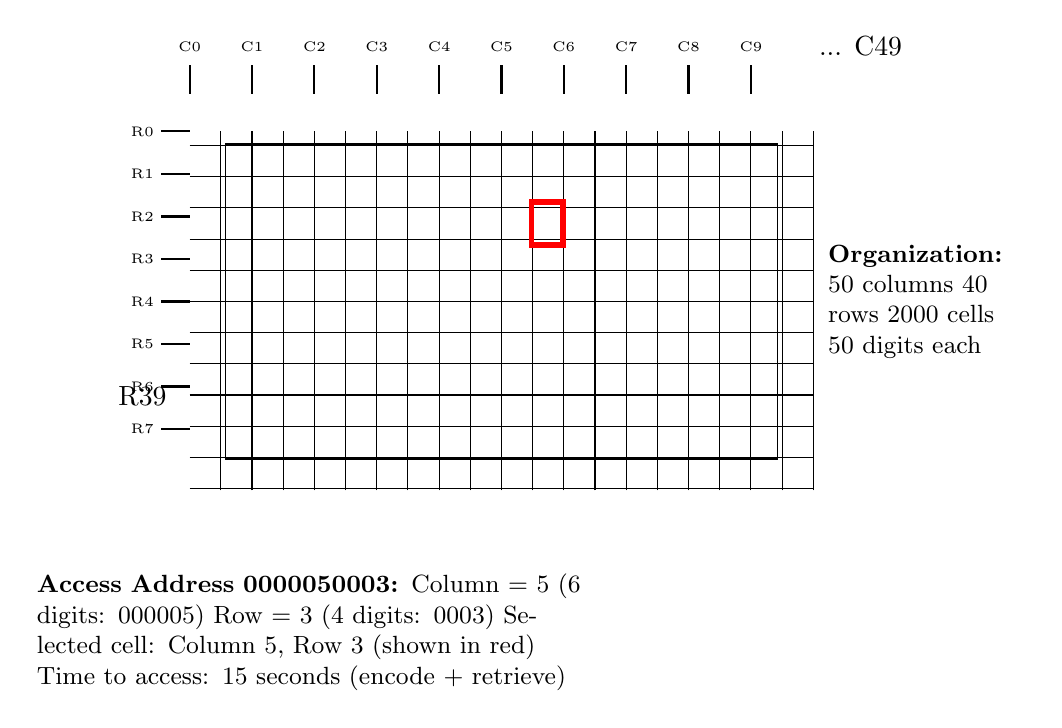
\begin{tikzpicture}[scale=1.2]

% Memory matrix (simplified view)
\node[draw, rectangle, minimum width=7cm, minimum height=4cm] (store) at (0, 0) {};

% Column selectors (top)
\foreach \i in {0,1,2,...,9} {
  \pgfmathsetmacro{\x}{-3.3 + 0.66*\i}
  \draw[thick] (\x, 2.2) -- (\x, 2.5);
  \node[draw=none, font=\tiny] at (\x, 2.7) {C\i};
}
\node[draw=none] at (3.8, 2.7) {... C49};

% Row selectors (left)
\foreach \i in {0,1,2,...,7} {
  \pgfmathsetmacro{\y}{1.8 - 0.45*\i}
  \draw[thick] (-3.6, \y) -- (-3.3, \y);
  \node[draw=none, font=\tiny] at (-3.8, \y) {R\i};
}
\node[draw=none] at (-3.8, -1.0) {R39};

% Grid of cells
\draw[step=0.33cm] (-3.3, -2.0) grid (3.3, 1.8);

% Highlight example cell at C5, R3
\draw[line width=2pt, red] (0.32, 1.05) rectangle (0.65, 0.6);

% Label
\node[draw=none] at (4.5, 0) [text width=2.5cm, font=\small] {
\textbf{Organization:}
50 columns
40 rows
2000 cells
50 digits each
};

% Access example
\node[draw=none] at (-2, -3.5) [text width=7cm, font=\small] {
\textbf{Access Address 0000050003:}
Column = 5 (6 digits: 000005)
Row = 3 (4 digits: 0003)
Selected cell: Column 5, Row 3 (shown in red)
Time to access: 15 seconds (encode + retrieve)
};

\end{tikzpicture}
\end{center}

\newpage

\section{The Barrel: Program Control Mechanism}

\begin{center}
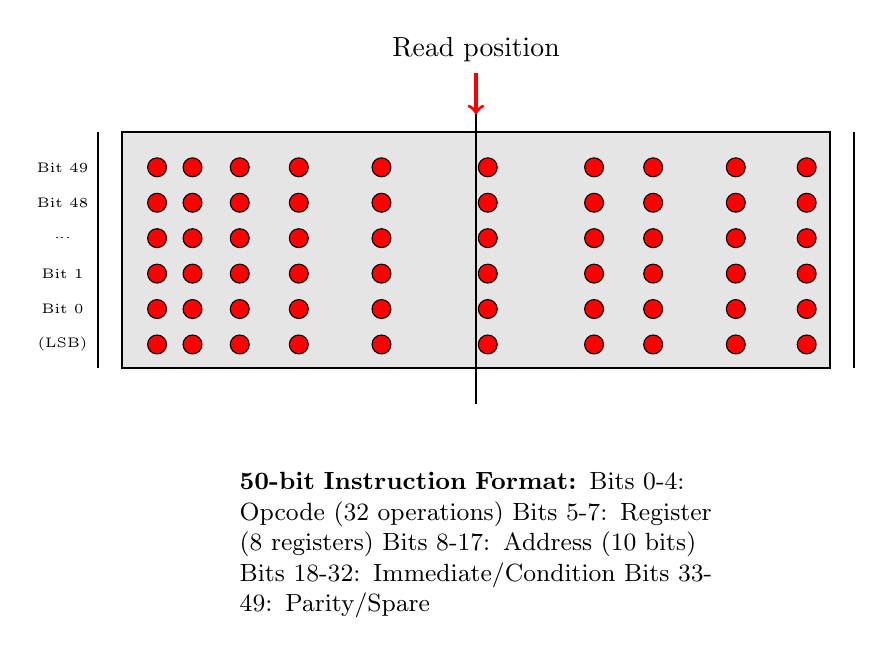
\begin{tikzpicture}[scale=1.5]

% Barrel cylinder (side view)
\draw[fill=gray!20, thick] (0, -1) rectangle (6, 1);
\draw[thick] (-0.2, -1) -- (-0.2, 1);
\draw[thick] (6.2, -1) -- (6.2, 1);

% Barrel axis
\draw[thick] (3, -1.3) -- (3, 1.3);

% Program pegs on barrel surface
\foreach \x in {0.3, 0.6, 1.0, 1.5, 2.2, 3.1, 4.0, 4.5, 5.2, 5.8} {
  \foreach \y in {-0.8, -0.5, -0.2, 0.1, 0.4, 0.7} {
    \draw[fill=red] (\x, \y) circle (0.08cm);
  }
}

% Track labels on left
\node[draw=none, font=\tiny] at (-0.5, 0.7) {Bit 49};
\node[draw=none, font=\tiny] at (-0.5, 0.4) {Bit 48};
\node[draw=none, font=\tiny] at (-0.5, 0.1) {···};
\node[draw=none, font=\tiny] at (-0.5, -0.2) {Bit 1};
\node[draw=none, font=\tiny] at (-0.5, -0.5) {Bit 0};
\node[draw=none, font=\tiny] at (-0.5, -0.8) {(LSB)};

% Position marker
\draw[->, very thick, red] (3, 1.5) -- (3, 1.15);
\node[draw=none] at (3, 1.7) {Read position};

% Instruction encoding
\node[draw=none, text width=6cm, font=\small] at (3, -2.5) {
\textbf{50-bit Instruction Format:}
Bits 0-4: Opcode (32 operations)
Bits 5-7: Register (8 registers)
Bits 8-17: Address (10 bits)
Bits 18-32: Immediate/Condition
Bits 33-49: Parity/Spare
};

\end{tikzpicture}
\end{center}

\newpage

\section{Carry Mechanism Detail}

\begin{center}
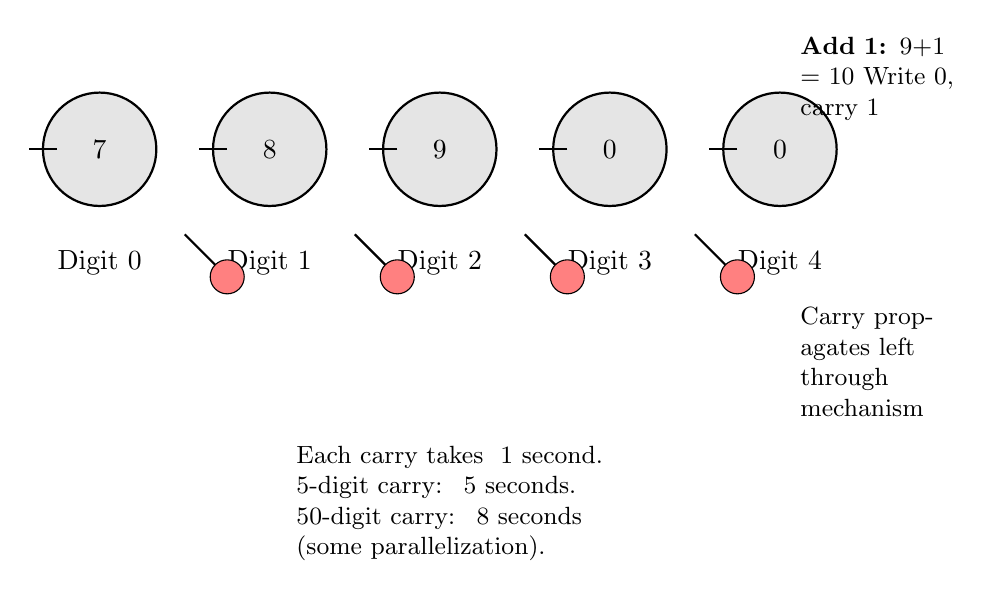
\begin{tikzpicture}[scale=1.8]

% Five consecutive digit wheels
\foreach \i in {0,1,2,3,4} {
  \pgfmathsetmacro{\x}{\i * 1.2}

  % Wheel
  \draw[fill=gray!20, thick] (\x, 0) circle (0.4cm);
  \draw[thick] (\x - 0.3, 0) -- (\x - 0.5, 0);

  % Digit value (varies)
  \ifnum \i=0 \node[draw=none] at (\x, 0) {7}; \fi
  \ifnum \i=1 \node[draw=none] at (\x, 0) {8}; \fi
  \ifnum \i=2 \node[draw=none] at (\x, 0) {9}; \fi
  \ifnum \i=3 \node[draw=none] at (\x, 0) {0}; \fi
  \ifnum \i=4 \node[draw=none] at (\x, 0) {0}; \fi

  % Label
  \ifnum \i=0 \node[draw=none] at (\x, -0.8) {Digit 0}; \fi
  \ifnum \i=1 \node[draw=none] at (\x, -0.8) {Digit 1}; \fi
  \ifnum \i=2 \node[draw=none] at (\x, -0.8) {Digit 2}; \fi
  \ifnum \i=3 \node[draw=none] at (\x, -0.8) {Digit 3}; \fi
  \ifnum \i=4 \node[draw=none] at (\x, -0.8) {Digit 4}; \fi
}

% Carry levers (below wheels)
\foreach \i in {0,1,2,3} {
  \pgfmathsetmacro{\x}{\i * 1.2 + 0.6}
  \draw[thick] (\x, -0.6) -- (\x + 0.3, -0.9);
  \draw[fill=red!50] (\x + 0.3, -0.9) circle (0.12cm);
}

% Annotations
\node[draw=none, text width=2cm, font=\small] at (5.5, 0.5) {
\textbf{Add 1:}
9+1 = 10
Write 0, carry 1
};

\node[draw=none, text width=2cm, font=\small] at (5.5, -1.5) {
Carry propagates
left through
mechanism
};

% Time annotation
\node[draw=none, text width=4cm, font=\small] at (2.5, -2.5) {
Each carry takes ~1 second.
5-digit carry: ~5 seconds.
50-digit carry: ~8 seconds (some parallelization).
};

\end{tikzpicture}
\end{center}

\newpage

\section{Pipe Buffer Mechanism (Rotating Drum)}

\begin{center}
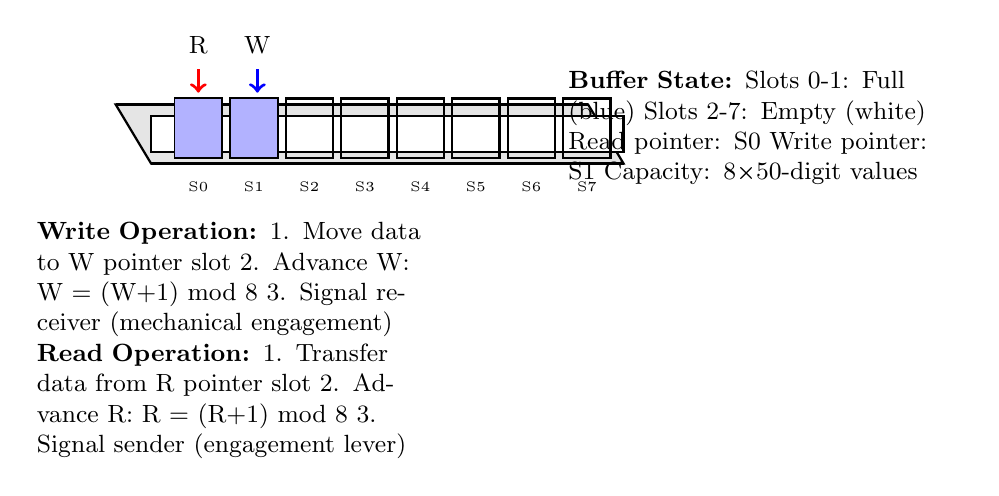
\begin{tikzpicture}[scale=1.5]

% Pipe buffer drum (side view)
\draw[fill=gray!20, thick] (0, 0) -- (0.3, -0.5) -- (4.3, -0.5) -- (4, 0) -- cycle;
\draw[thick] (0, 0) -- (4, 0);
\draw[thick] (0.3, -0.5) -- (4.3, -0.5);

% Rotating cylinder representation
\draw[fill=white, thick] (0.3, -0.1) rectangle (4.3, -0.4);

% 8 data slots shown from top
\foreach \i in {0,1,2,3,4,5,6,7} {
  \pgfmathsetmacro{\x}{0.5 + \i * 0.47}

  % Slot rectangle
  \draw[thick] (\x, 0.05) rectangle (\x + 0.4, -0.45);

  % Fill some slots to show data
  \ifnum \i<2
    \draw[fill=blue!30] (\x, 0.05) rectangle (\x + 0.4, -0.45);
  \fi

  \node[draw=none, font=\tiny] at (\x + 0.2, -0.7) {S\i};
}

% Read/Write pointers
\draw[->, very thick, red] (0.7, 0.3) -- (0.7, 0.1);
\node[draw=none] at (0.7, 0.5) {\small R};

\draw[->, very thick, blue] (1.2, 0.3) -- (1.2, 0.1);
\node[draw=none] at (1.2, 0.5) {\small W};

% Legend
\node[draw=none, text width=5cm, font=\small] at (5.5, -0.2) {
\textbf{Buffer State:}
Slots 0-1: Full (blue)
Slots 2-7: Empty (white)
Read pointer: S0
Write pointer: S1
Capacity: 8×50-digit values
};

% Operation detail
\node[draw=none, text width=5cm, font=\small] at (1, -2) {
\textbf{Write Operation:}
1. Move data to W pointer slot
2. Advance W: W = (W+1) mod 8
3. Signal receiver (mechanical engagement)

\textbf{Read Operation:}
1. Transfer data from R pointer slot
2. Advance R: R = (R+1) mod 8
3. Signal sender (engagement lever)
};

\end{tikzpicture}
\end{center}

\newpage

\section{Process Management: In-Memory Process Table}

\begin{center}
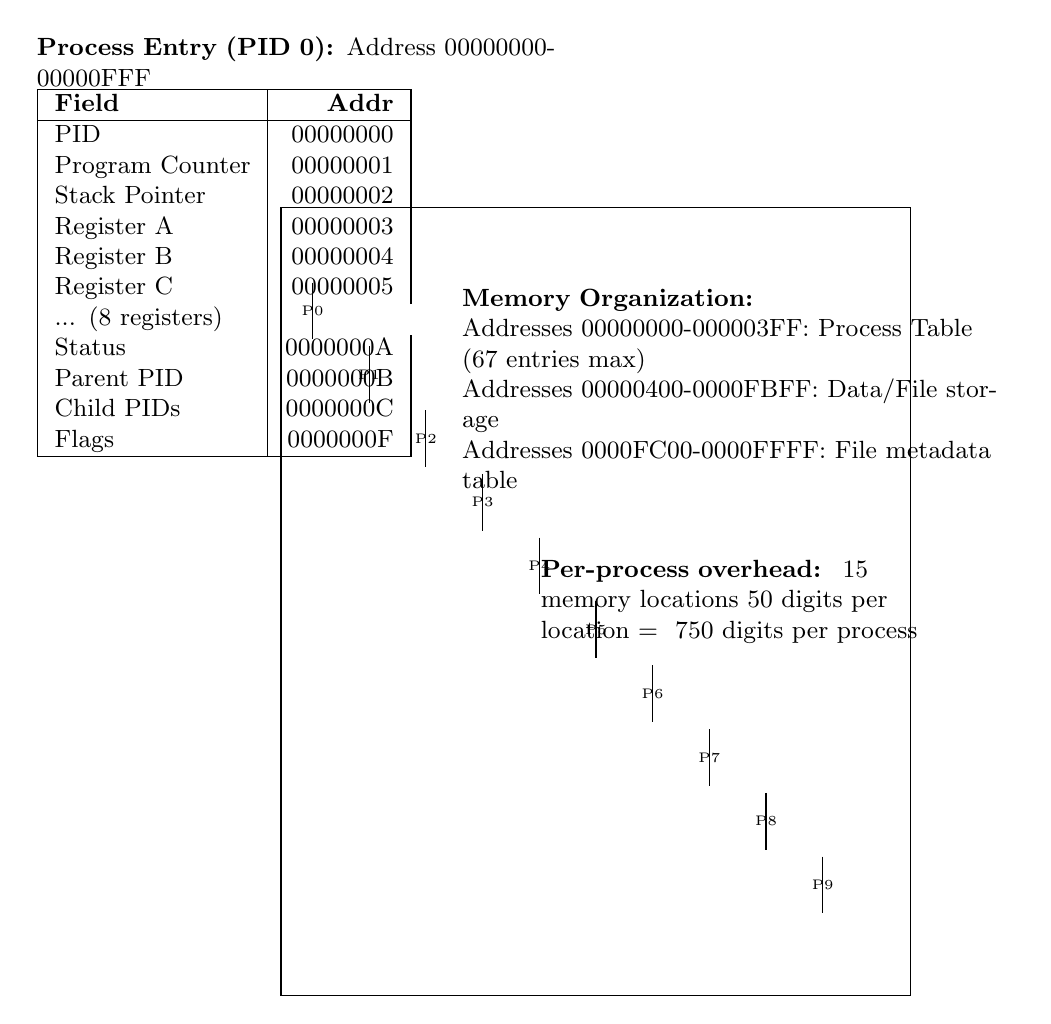
\begin{tikzpicture}[scale=0.9]

% Memory layout
\node[draw, rectangle, minimum width=8cm, minimum height=10cm] (mem) at (0, 0) {};

% Process entries
\foreach \i in {0,1,2,...,9} {
  \pgfmathsetmacro{\y}{4.5 - \i * 0.9}
  \draw (\i*0.8 - 4, \y) -- (\i*0.8 - 4, \y - 0.8);
  \node[draw=none, font=\tiny] at (\i*0.8 - 4, \y - 0.4) {P\i};
}

% Detailed process entry structure (first process)
\node[draw=none] at (-4, 5) [text width=7cm, font=\small] {
\textbf{Process Entry (PID 0):}
Address 00000000-00000FFF

\begin{tabular}{|l|r|}
\hline
\textbf{Field} & \textbf{Addr} \\
\hline
PID & 00000000 \\
Program Counter & 00000001 \\
Stack Pointer & 00000002 \\
Register A & 00000003 \\
Register B & 00000004 \\
Register C & 00000005 \\
... (8 registers) \\
Status & 0000000A \\
Parent PID & 0000000B \\
Child PIDs & 0000000C \\
Flags & 0000000F \\
\hline
\end{tabular}
};

% Memory regions annotation
\node[draw=none, text width=7cm, font=\small] at (2, 3) {
\textbf{Memory Organization:}

Addresses 00000000-000003FF:
Process Table (67 entries max)

Addresses 00000400-0000FBFF:
Data/File storage

Addresses 0000FC00-0000FFFF:
File metadata table
};

% Per-process size calculation
\node[draw=none, text width=5cm, font=\small] at (2, 0) {
\textbf{Per-process overhead:}
~15 memory locations
50 digits per location
= ~750 digits per process
};

\end{tikzpicture}
\end{center}

\newpage

\section{Execution Timeline: Simple Program}

\begin{center}
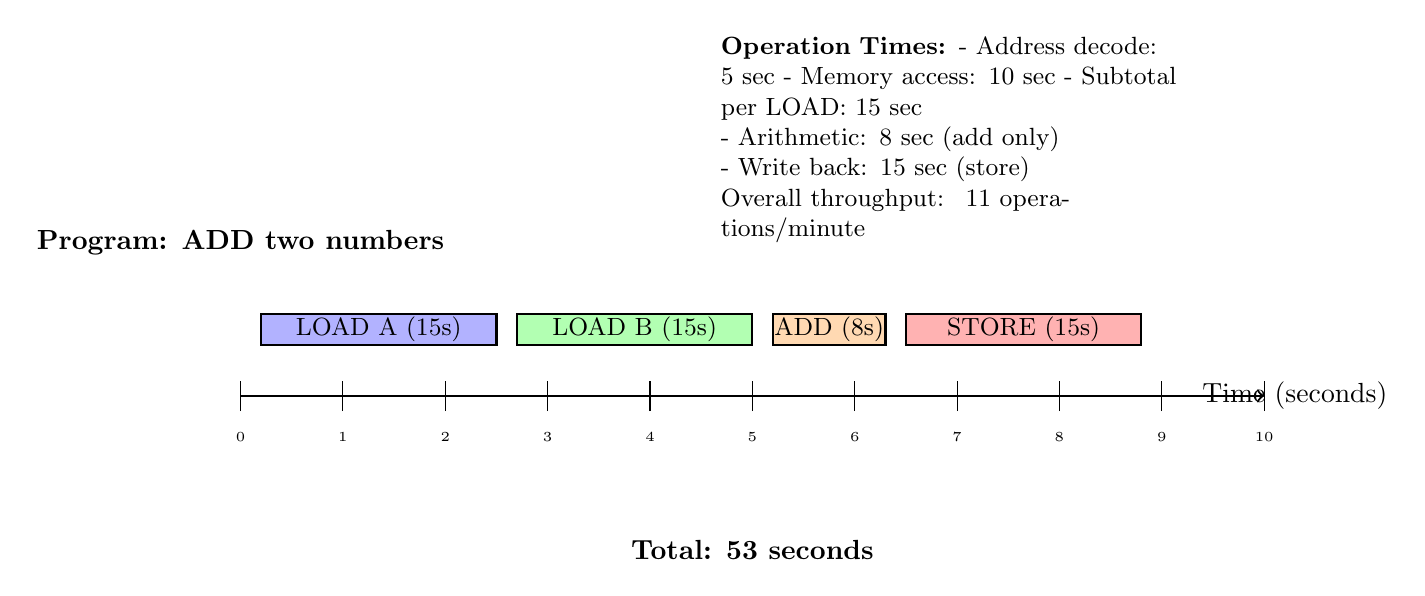
\begin{tikzpicture}[scale=1.3]

% Time axis
\draw[->,thick] (0, 0) -- (10, 0);
\node[draw=none] at (10.3, 0) {Time (seconds)};

% Program steps
\node[draw=none] at (0, 1.5) {\textbf{Program: ADD two numbers}};

% Instruction 1: LOAD A
\draw[fill=blue!30, thick] (0.2, 0.5) rectangle (2.5, 0.8);
\node[draw=none, font=\small] at (1.35, 0.65) {LOAD A (15s)};

% Instruction 2: LOAD B
\draw[fill=green!30, thick] (2.7, 0.5) rectangle (5, 0.8);
\node[draw=none, font=\small] at (3.85, 0.65) {LOAD B (15s)};

% Instruction 3: ADD
\draw[fill=orange!30, thick] (5.2, 0.5) rectangle (6.3, 0.8);
\node[draw=none, font=\small] at (5.75, 0.65) {ADD (8s)};

% Instruction 4: STORE
\draw[fill=red!30, thick] (6.5, 0.5) rectangle (8.8, 0.8);
\node[draw=none, font=\small] at (7.65, 0.65) {STORE (15s)};

% Time markers
\foreach \t in {0,1,2,3,4,5,6,7,8,9,10} {
  \draw (\t, -0.15) -- (\t, 0.15);
  \node[draw=none, font=\tiny] at (\t, -0.4) {\t};
}

% Total time
\node[draw=none] at (5, -1.5) {\textbf{Total: 53 seconds}};

% Detailed breakdown
\node[draw=none, text width=6cm, font=\small] at (7, 2.5) {
\textbf{Operation Times:}
- Address decode: 5 sec
- Memory access: 10 sec
- Subtotal per LOAD: 15 sec

- Arithmetic: 8 sec (add only)

- Write back: 15 sec (store)

Overall throughput:
~11 operations/minute
};

\end{tikzpicture}
\end{center}

\newpage

\section{Performance Comparison: Operation Times}

\begin{center}
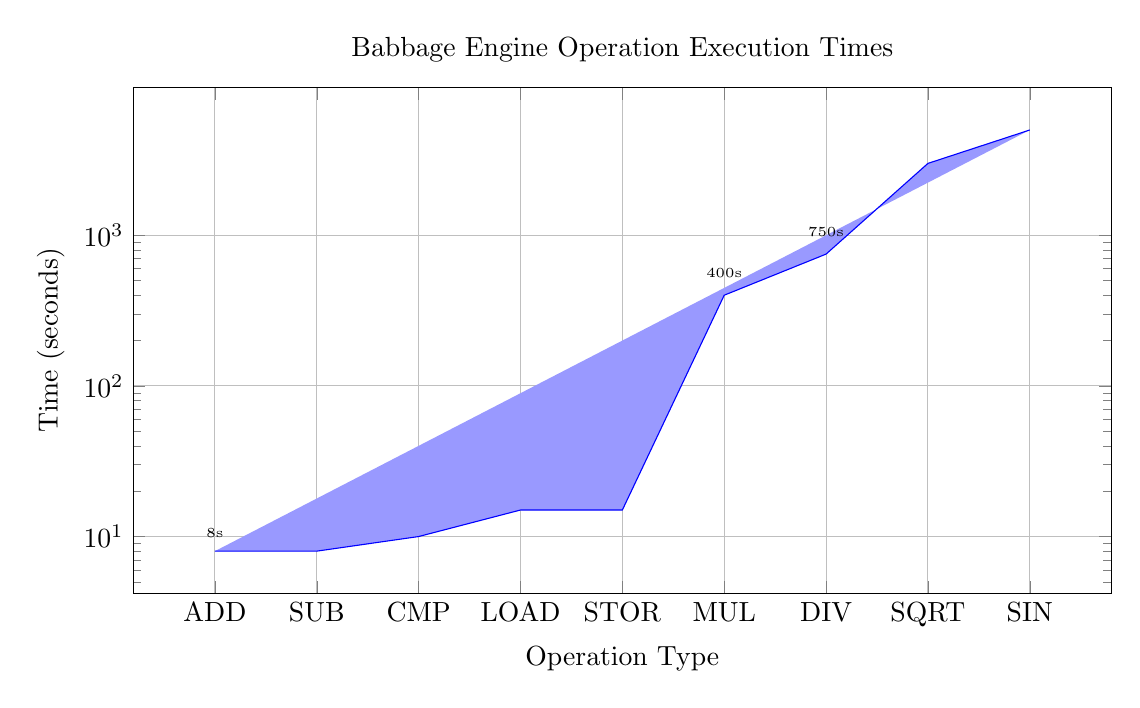
\begin{tikzpicture}
\begin{axis}[
  title={Babbage Engine Operation Execution Times},
  xlabel={Operation Type},
  ylabel={Time (seconds)},
  ymode=log,
  ytick={1,10,100,1000},
  grid=major,
  bar width=0.6cm,
  width=14cm,
  height=8cm,
  xtick={0,1,2,3,4,5,6,7,8},
  xticklabels={ADD, SUB, CMP, LOAD, STOR, MUL, DIV, SQRT, SIN},
]

\addplot[fill=blue!40, draw=blue] coordinates {
  (0, 8)      % ADD
  (1, 8)      % SUB
  (2, 10)     % CMP
  (3, 15)     % LOAD
  (4, 15)     % STOR
  (5, 400)    % MUL (50×50)
  (6, 750)    % DIV
  (7, 3000)   % SQRT
  (8, 5000)   % SIN
};

% Annotations
\node[draw=none, anchor=south] at (0, 8.5) {\tiny 8s};
\node[draw=none, anchor=south] at (5, 450) {\tiny 400s};
\node[draw=none, anchor=south] at (6, 850) {\tiny 750s};

\end{axis}
\end{tikzpicture}
\end{center}

\newpage

\section{Unix to Mechanical Mapping Table}

\begin{center}
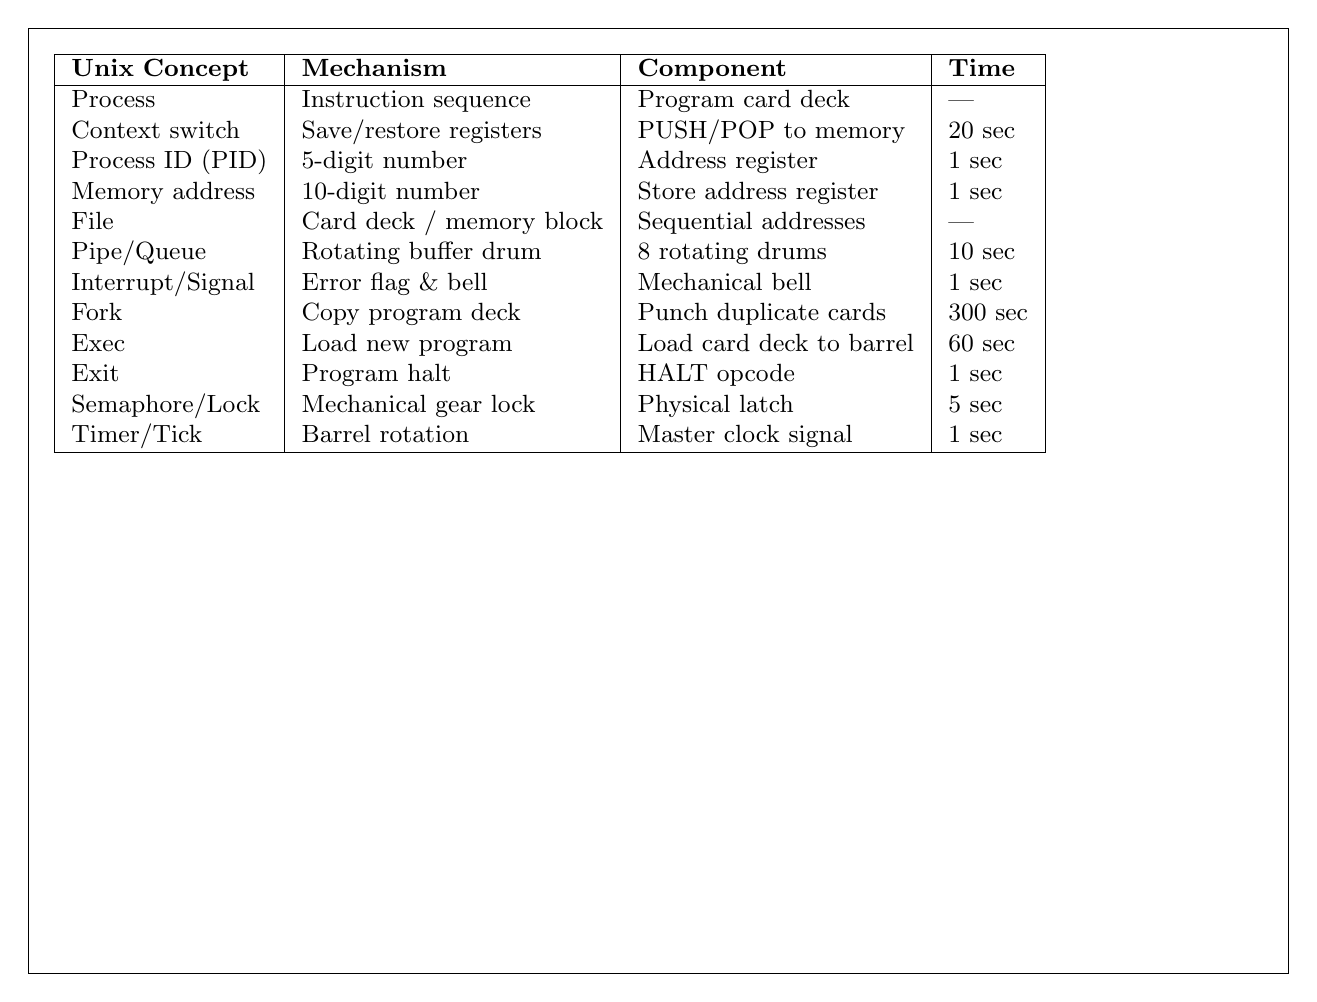
\begin{tikzpicture}

\node[draw, rectangle, minimum width=16cm, minimum height=12cm] (table) at (0, 0) {};

\node[draw=none, anchor=north west, text width=15cm, font=\small] at (-7.8, 5.8) {
\begin{tabular}{|l|l|l|l|}
\hline
\textbf{Unix Concept} & \textbf{Mechanism} & \textbf{Component} & \textbf{Time} \\
\hline
Process & Instruction sequence & Program card deck & — \\
Context switch & Save/restore registers & PUSH/POP to memory & 20 sec \\
Process ID (PID) & 5-digit number & Address register & 1 sec \\
Memory address & 10-digit number & Store address register & 1 sec \\
File & Card deck / memory block & Sequential addresses & — \\
Pipe/Queue & Rotating buffer drum & 8 rotating drums & 10 sec \\
Interrupt/Signal & Error flag \& bell & Mechanical bell & 1 sec \\
Fork & Copy program deck & Punch duplicate cards & 300 sec \\
Exec & Load new program & Load card deck to barrel & 60 sec \\
Exit & Program halt & HALT opcode & 1 sec \\
Semaphore/Lock & Mechanical gear lock & Physical latch & 5 sec \\
Timer/Tick & Barrel rotation & Master clock signal & 1 sec \\
\hline
\end{tabular}
};

\end{tikzpicture}
\end{center}

\newpage

\section{Physical Machine Layout (Bird's Eye View)}

\begin{center}
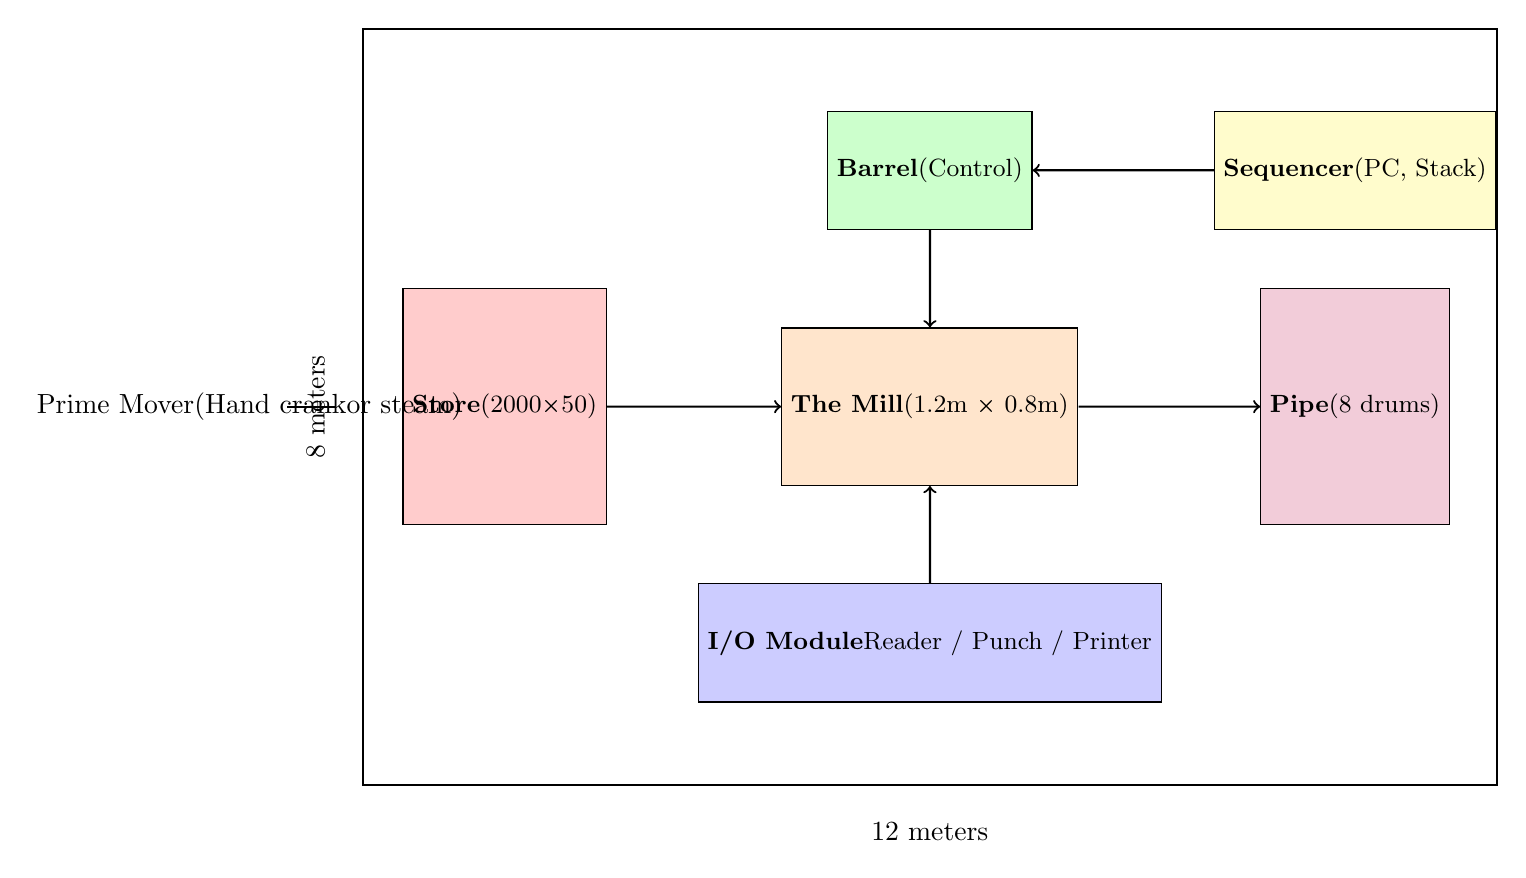
\begin{tikzpicture}[scale=1.2]

% Floor plan outline
\draw[thick] (0, 0) rectangle (12, 8);

% The Mill (center)
\node[draw, rectangle, minimum width=3cm, minimum height=2cm, fill=orange!20] (mill) at (6, 4) {
  \small \textbf{The Mill}\\(1.2m × 0.8m)
};

% The Store (left side)
\node[draw, rectangle, minimum width=2cm, minimum height=3cm, fill=red!20] (store) at (1.5, 4) {
  \small \textbf{Store}\\(2000×50)
};

% The Barrel (top)
\node[draw, rectangle, minimum width=2cm, minimum height=1.5cm, fill=green!20] (barrel) at (6, 6.5) {
  \small \textbf{Barrel}\\(Control)
};

% I/O Module (bottom)
\node[draw, rectangle, minimum width=4cm, minimum height=1.5cm, fill=blue!20] (io) at (6, 1.5) {
  \small \textbf{I/O Module}\\Reader / Punch / Printer
};

% Pipe buffers (right side)
\node[draw, rectangle, minimum width=2cm, minimum height=3cm, fill=purple!20] (pipes) at (10.5, 4) {
  \small \textbf{Pipe}\\(8 drums)
};

% Process Sequencer (top right)
\node[draw, rectangle, minimum width=2cm, minimum height=1.5cm, fill=yellow!20] (seq) at (10.5, 6.5) {
  \small \textbf{Sequencer}\\(PC, Stack)
};

% Connections
\draw[->,thick] (store) -- (mill);
\draw[->,thick] (barrel) -- (mill);
\draw[->,thick] (mill) -- (pipes);
\draw[->,thick] (io) -- (mill);
\draw[->,thick] (seq) -- (barrel);

% Dimensions
\node[draw=none] at (6, -0.5) {12 meters};
\node[draw=none] at (-0.5, 4) {\rotatebox{90}{8 meters}};

% Power input
\draw[thick] (-0.3, 4) -- (-0.8, 4);
\node[draw=none] at (-1.2, 4) {Prime Mover\\(Hand crank\\or steam)};

\end{tikzpicture}
\end{center}

\newpage

\section{Instruction Format (50 bits)}

\begin{center}
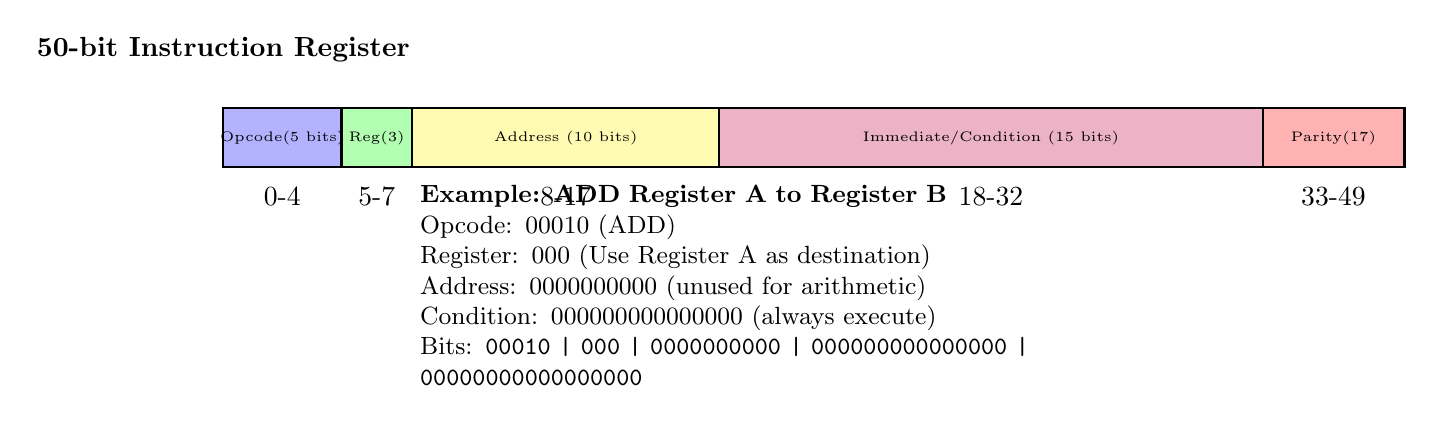
\begin{tikzpicture}[scale=1.5]

% Instruction register visualization
\node[draw=none] at (0, 2) {\textbf{50-bit Instruction Register}};

% Bit fields
\draw[thick] (0, 1.5) rectangle (10, 1);

% Opcode (bits 0-4)
\draw[fill=blue!30, thick] (0, 1.5) rectangle (1, 1);
\node[draw=none] at (0.5, 1.25) {\tiny Opcode\\(5 bits)};
\node[draw=none] at (0.5, 0.75) {0-4};

% Register (bits 5-7)
\draw[fill=green!30, thick] (1, 1.5) rectangle (1.6, 1);
\node[draw=none] at (1.3, 1.25) {\tiny Reg\\(3)};
\node[draw=none] at (1.3, 0.75) {5-7};

% Address (bits 8-17)
\draw[fill=yellow!30, thick] (1.6, 1.5) rectangle (4.2, 1);
\node[draw=none] at (2.9, 1.25) {\tiny Address (10 bits)};
\node[draw=none] at (2.9, 0.75) {8-17};

% Immediate/Condition (bits 18-32)
\draw[fill=purple!30, thick] (4.2, 1.5) rectangle (8.8, 1);
\node[draw=none] at (6.5, 1.25) {\tiny Immediate/Condition (15 bits)};
\node[draw=none] at (6.5, 0.75) {18-32};

% Parity/Spare (bits 33-49)
\draw[fill=red!30, thick] (8.8, 1.5) rectangle (10, 1);
\node[draw=none] at (9.4, 1.25) {\tiny Parity\\(17)};
\node[draw=none] at (9.4, 0.75) {33-49};

% Example instruction
\node[draw=none, text width=10cm, font=\small] at (5, 0) {
\textbf{Example: ADD Register A to Register B}\\
Opcode: 00010 (ADD)\\
Register: 000 (Use Register A as destination)\\
Address: 0000000000 (unused for arithmetic)\\
Condition: 000000000000000 (always execute)\\
Bits: \texttt{00010 | 000 | 0000000000 | 000000000000000 | 00000000000000000}
};

\end{tikzpicture}
\end{center}

\end{document}
